\documentclass[twoside]{homework}

% for bar over variable
\newcommand*\conj[1]{\overline{#1}}
\newcommand*\mean[1]{\overline{#1}}

% for graph
\usepackage{pgfplots}
\usepackage{enumerate}
% for double stroke 1
\usepackage{bbm}

% for < and >
\usepackage[T1]{fontenc}
\usepackage{tikz}
\usetikzlibrary{arrows.meta}
% for equation wrap text
\usepackage{amsmath}
\usepackage{bm}

\studname{Kangwei Ling}
\studmail{kl3076@columbia.edu}
\coursename{CSOR 4231, Section 3: Analysis of Algorithms I}
\hwNo{3}
\begin{document}
\maketitle
\subsubsection*{Collaborators}
Zefeng Liu (zl2715), Kunyan Han (kh2931), Luoyao Hao (lh2913).

\section{DPV 3.1}
See below.\\
\includegraphics[width=.5\textwidth]{3-1.png}

\section{DPV 3.21}
We can modify the existing linear time algorithm for finding all strongly connected component algorithm to do this:

\begin{enumerate}
	\item Each time we find a "sink" SCC (a source in the reversed graph), we run a modified version of DFS on the SCC:
		\begin{enumerate}
			\item We begin the DFS at any vertex $s$, it will reach all vertices in this SCC for sure.
			\item We do not use $visited$ but rather give each vertex a color (red or black), we give $s$ red. And each time we go on an edge $(u, v)$, we assign red to $v$ if $u$ is black, otherwise black.
			\item At some point, we run in to an edge $(u, v)$ and $v$ have already been colored. If $color(u) \neq color(v)$, we view this as we have already visited $v$, just backtrack to other edges. If $color(u) = color(v)$, then we can discover an odd length cycle around vertices $u, v$, we can goto step 2.
			\item If the DFS ends and we have not ran into any edge $(u, v)$ such that $color(u) = color(v)$, we need to try the next "sink" SCC.
		\end{enumerate}
	\item If we find $(u, v)$ that $color(u) = color(v)$, suppose the path we found when coloring is $s \leadsto u$ and $s \leadsto v$, then either the length of these two path is both even or both odd (since they have the same color).

	If they are even, we run DFS from $v$ to find a path $v \leadsto s$, the path exists because they are in the same SCC. If the length of $v \leadsto s$ is even, then cycle $s \leadsto u \rightarrow v \leadsto s$ is an odd cycle. Otherwise, $s\leadsto v \leadsto s$ is an odd cycle.

	If they are odd, we run DFS from $v$ to find a path $v \leadsto s$. If the length of $v \leadsto s$ is odd, then cycle $s \leadsto u \rightarrow v \leadsto s$ is an odd cycle. Otherwise, $s\leadsto v \leadsto s$ is an odd cycle.
\end{enumerate}

Note that, the modified SCC algorithm in step 1 still runs in linear time, and step 2 also runs in linear time.

\section{DPV 3.28}
\begin{enumerate}
	\item [(a)] set $x_1, x_2, x_3, x_4$ to true, true, false, true also satisfy this 2SAT.
	\item [(b)] $(x_1 \lor x_2) \land (x_1 \lor \bar{x}_2) \land (\bar{x}_1 \lor \bar{x}_3) \land (\bar{x}_1 \lor x_3) \land (x_3 \lor x_4)$

	\item [(c)] For the instance given in the problem: \\
	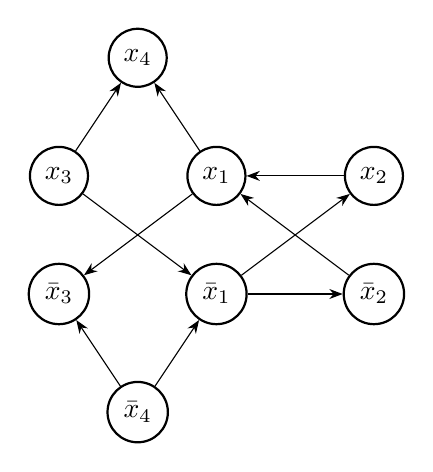
\begin{tikzpicture}
		\begin{scope}[every node/.style={circle,thick,draw}]
			\node (x1) at (0,0) {$x_1$};
			\node (x1b) at (0,-1.5) {$\bar{x}_1$};

			\node (x2) at (2,0) {$x_2$};
			\node (x2b) at (2,-1.5) {$\bar{x}_2$};

			\node (x3) at (-2,0) {$x_3$};
			\node (x3b) at (-2,-1.5) {$\bar{x}_3$};

			\node (x4) at (-1,1.5) {$x_4$};
			\node (x4b) at (-1,-3) {$\bar{x}_4$};

		\end{scope}

		\begin{scope}[>={Stealth[black]},
					  every node/.style={fill=white,circle},
					  every edge/.style={draw=black}]
			\path [->] (x1b) edge (x2b);
			\path [->] (x2) edge (x1);

			\path [->] (x1) edge (x3b);
			\path [->] (x3) edge (x1b);

			\path [->] (x1b) edge (x2);
			\path [->] (x2b) edge (x1);

			\path [->] (x3) edge (x4);
			\path [->] (x4b) edge (x3b);

			\path [->] (x1) edge (x4);
			\path [->] (x4b) edge (x1b);

			%\path [->] (x1b) edge node (x2b);
%			\path [->] (B) edge[bend right=60] node {$1$} (E);
		\end{scope}
		\end{tikzpicture}

		For the instance in (b): \\
	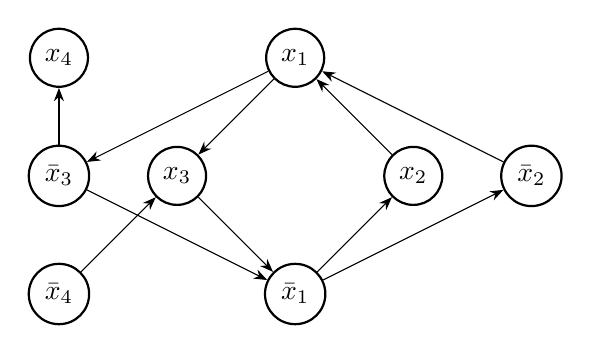
\begin{tikzpicture}
		\begin{scope}[every node/.style={circle,thick,draw}]
			\node (x1) at (0,0) {$x_1$};
			\node (x1b) at (0,-3) {$\bar{x}_1$};

			\node (x2) at (1.5,-1.5) {$x_2$};
			\node (x2b) at (3,-1.5) {$\bar{x}_2$};

			\node (x3) at (-1.5,-1.5) {$x_3$};
			\node (x3b) at (-3,-1.5) {$\bar{x}_3$};

			\node (x4) at (-3, 0) {$x_4$};
			\node (x4b) at (-3,-3) {$\bar{x}_4$};

		\end{scope}

		\begin{scope}[>={Stealth[black]},
					  every node/.style={fill=white,circle},
					  every edge/.style={draw=black}]
			\path [->] (x1b) edge (x2);
			\path [->] (x2b) edge (x1);

			\path [->] (x1b) edge (x2b);
			\path [->] (x2) edge (x1);

			\path [->] (x1) edge (x3b);
			\path [->] (x3) edge (x1b);

			\path [->] (x1) edge (x3);
			\path [->] (x3b) edge (x1b);

			\path [->] (x3b) edge (x4);
			\path [->] (x4b) edge (x3);

			%\path [->] (x1b) edge node (x2b);
%			\path [->] (B) edge[bend right=60] node {$1$} (E);
		\end{scope}
		\end{tikzpicture}

		\newcommand{\xbar}{\bar{x}}
		\newcommand{\ubar}{\bar{u}}
		\newcommand{\vbar}{\bar{v}}
		\item [(d)] If $G_I$ has a strongly connected component containing both $x$ and $\bar{x}$ for some variable $x$. Since they are in a strongly connected component, there's path from $x$ to $\bar{x}$ and vice versa. Let's say $x  \leadsto u_1 \leadsto \cdots \leadsto u_i \leadsto \bar{x} $ and $\bar{x}  \leadsto v_1 \leadsto \cdots \leadsto v_j \leadsto x$ are the paths in the SCC.

		From the method that we used to construct the graph $G_I$, we know that for these two path to exists, the 2SAT must have the following two parts:
		\begin{align}
			(\xbar \lor u_1) \land (\ubar_1 \lor u_2) \land \cdots \land (\ubar_i \lor \xbar) \label{eq:term1}\\
			(x \lor v_1) \land (\vbar_1 \lor v_2) \land \cdots \land (\vbar_j \lor x) \label{eq:term2}
		\end{align}
		To satisfy the 2SAT, both \ref{eq:term1} and \ref{eq:term2} need to be satisfied. If we assign true to $x$, thus $\bar{x}$ is false, then in order to satisfy \ref{eq:term1}, the first clause implies $u_1$ must be true, then $u_2$ must be true to satisfy the second clause, keep going on, to the very end, we have that $\bar{x}$ must be true, which is impossible since $x$ is true.

		In the same way, if we assign false to $x$, we cannot satisfy \ref{eq:term2}.

		$x$ must be true or false anyway, in either way, we cannot satisfy both \ref{eq:term1} and \ref{eq:term2}. But they are all part of the 2SAT we are trying to satisfy, therefore, $I$ has no satisfying assignment.

		\item [(e)] It is obvious that each clause is translated into 2 edges in $G_I$, to satisfy an instance $I$ is to satisfy every edge of $G_I$. Here we define that to satisfy an edge is to satisfy the clause it implies by assigning true or false to each side of the edge. To be clear, for any edge $(u, v)$ in $G_I$, to satisfy this edge means by assigning true or false to $u, v$, we make $(\ubar \lor v)$ evaluate to true. (here $u, v$ can be variables or negations). Note that the other edge $(\vbar, \ubar)$ is satisfied automatically because they are from the same clause.

		To see that "if none of $G_I$'s SCCs contain both a literal and its negation, then the instance $I$ must be satisfiable", we must show that we can satisfy every edge in this case.

		We can proceed by repeatedly picking a sink strongly connected component $S$ of $G_I$ and make assignment to nodes inside it. The assignment are as follows:
		\begin{itemize}
			\item For each node $u$ in $S$, if $u$ contains variable that we haven't assigned yet (I call it \textbf{fresh node} below), we assign the variable to make $u$ true. That is, if $u = x$, we assign $x = true$, otherwise $x = false$.
			\item If $u$ contains variable that is already assigned (we meet the $\ubar$ one earlier), we leave it be.
		\end{itemize}
		Proceed like this will give us the assignment of variables that satisfy the instance $I$ because:
		\begin{itemize}
			\item An edge $(u, v)$ is satisfied if either $v = true$ or $u = false$, since $(u, v)$ implies $(\ubar \lor v)$.
			\item Every edge $(u, v)$ in a SCC($u, v$ are in the same SCC) is satisfied after we make assignments to its nodes.
				\begin{enumerate}
					\item if $v$ is a fresh node, then by assignment, $v = true$, this edge is satisfied.
					\item if $v$ is not a fresh node, then $u$ is also not one, because $(u, v)$ implies $(\ubar \lor v)$, another equivalent edge is $(\vbar, \ubar)$. We must have encountered $\vbar$ in an earlier "sink" SCC, and either $\ubar$ is in the same SCC with $\vbar$ or it is in an even much earlier "sink" SCC. Either cases, $(\vbar, \ubar)$ must already been satisfied, thus $(u, v)$ is satisfied. (See below for how cross SCC edges are satisfied).
				\end{enumerate}

			\item Every cross SCC edge $(u, v)$ (where $u \in S, v \in S'$, $S, S'$ are different SCC in our proceeding order) is satisfied after $S, S'$ have all been processed.
				\begin{enumerate}
					\item Since edge $(u, v)$ exists, $S'$ becomes the sink earlier than $S$. Thus if $v$ is a fresh node, we must have assigned it true. Then $(u, v)$ is satisfied.
					\item If $v$ is not a fresh node, then just like edges in SCC, the other corresponding edge $(\vbar, \ubar)$ must have been satisfied.
				\end{enumerate}
		\end{itemize}
		From the explanation above we can conclude that we can satisfy all edges, therefore satisfy the instance $I$ with a set of assignments.

		\item [(f)] From class and also the textbook, we learnt a linear algorithm to find all strongly connected components of a graph by using a modified DFS algorithm on the graph and its reverse one. We can embed the procedure to give node true/false in (e) for each sinking component. Constant operations is added to process each node, therefore we have a linear time algorithm to solve 2SAT.
\end{enumerate}


\section{DPV 4.1}
\begin{enumerate}
	\item [(a)] See the table below.
	\begin{table}[!h]
		\centering
		\begin{tabular}{|l|l|l|l|l|l|l|l|l|}
		\hline
		iteration & A & B        & C        & D        & E        & F        & G        & H        \\ \hline
		initial   & 0 & $\infty$ & $\infty$ & $\infty$ & $\infty$ & $\infty$ & $\infty$ & $\infty$ \\ \hline
		1         & 0 & 1        & $\infty$ & $\infty$ & 4        & 8        & $\infty$ & $\infty$ \\ \hline
		2         & 0 & 1        & 3        & $\infty$ & 4        & 7        & 7        & $\infty$ \\ \hline
		3         & 0 & 1        & 3        & 4        & 4        & 7        & 5        & $\infty$ \\ \hline
		4         & 0 & 1        & 3        & 4        & 4        & 7        & 5        & 8        \\ \hline
		5         & 0 & 1        & 3        & 4        & 4        & 7        & 5        & 8        \\ \hline
		6         & 0 & 1        & 3        & 4        & 4        & 6        & 5        & 6        \\ \hline
		7         & 0 & 1        & 3        & 4        & 4        & 6        & 5        & 6        \\ \hline
		8         & 0 & 1        & 3        & 4        & 4        & 6        & 5        & 6        \\ \hline
		\end{tabular}
		\end{table}

	\item [(b)] Shortest-path tree: \\
	\begin{figure}[!h]
		\centering
	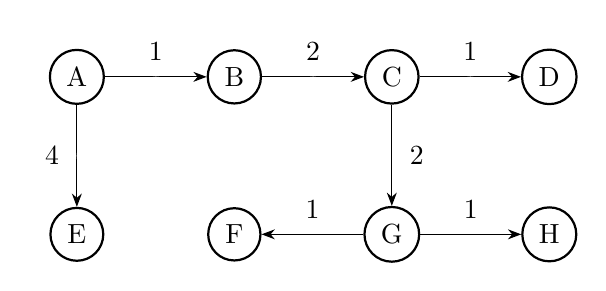
\begin{tikzpicture}
		\begin{scope}[every node/.style={circle,thick,draw}]
			\node (A) at (0,0) {A};
			\node (B) at (2,0) {B};
			\node (C) at (4,0) {C};
			\node (D) at (6,0) {D};

			\node (E) at (0,-2) {E};
			\node (F) at (2,-2) {F};
			\node (G) at (4,-2) {G};
			\node (H) at (6,-2) {H};


		\end{scope}

		\begin{scope}[>={Stealth[black]},
					  every node/.style={fill=white,circle},
					  every edge/.style={draw=black}]
			\path [->] (A) edge node [above] {1} (B);
			\path [->] (B) edge node [above] {2} (C);
			\path [->] (C) edge node [above] {1} (D);

			\path [->] (C) edge node [right] {2} (G);

			\path [->] (A) edge node [left] {4} (E);

			\path [->] (G) edge node [above] {1} (F);
			\path [->] (G) edge node [above] {1} (H);
			%\path [->] (x1b) edge node (x2b);
%			\path [->] (B) edge[bend right=60] node {$1$} (E);
		\end{scope}
		\end{tikzpicture}
	\end{figure}
\end{enumerate}

\section{}
\begin{enumerate}
	\item [(a)] we can modify the Dijkstra's algorithm to store the number of edges of it takes to go from the source node to this node via the current shortest path. Refering to Figure 4.8 in the textbook, we edit the testing

	\texttt{if dist(v) > dist(u) + l(u, v)}

	to

	\texttt{if (dist(v) > dist(u) + l(u, v)) or}

	\texttt{(dist(v) == dist(u) + l(u, v) and steps(v) > steps(u) + 1)}

	where \texttt{steps(u)} is the number of edges on the current shortest path from source to $u$.

	And when we update \texttt{dist(v)}, we also update \texttt{steps(v) = steps(u) + 1}

	\item [(b)] We can modify the weights of the edges to achieve this. Note that a path will be at most contain $|V| - 1$ edges. We can use $k$ bit to represent the number of edges in the path, $k$ is the minimum integer s.t. $x^k - 1 \leq |V| - 1$.

	We modify the weight of each edge like this: We left shift the weight by $k$ (equivalent to multiply by $2^k$), then add 1 to it.

	In this way, shorter path in the original graph is still shorter, since the weight is still dominated by the original weight. And path with same weight sum in original path will be different in lower $k$ bit, the path with fewest edges is shorter in this case.
\end{enumerate}


%\underline{Citation:} Please cite any sources you used for this problem.
\end{document}